\documentclass[12pt,a4paper]{article}

\usepackage{tikz}
\usetikzlibrary{graphs, graphs.standard, quotes}
\usetikzlibrary{positioning, arrows, automata}
\usepackage{tkz-berge}
\usepackage{graphicx}
\usepackage{caption}
\usepackage{subcaption}
\usepackage{tabularx}
\usepackage{algorithmic}
\usepackage{algorithm2e}
\usepackage[utf8]{inputenc}
\usepackage{wrapfig}
\usepackage{float}
\usepackage{etoolbox}

\renewcommand{\familydefault}{\rmdefault}

\BeforeBeginEnvironment{figure}{\vskip-2ex}
\AfterEndEnvironment{figure}{\vskip-2ex}

\begin{document}

\begin{titlepage}
	\centering
	\includegraphics[width=0.30\textwidth]{Teclogocompleto.jpg}\par\vspace{1cm}
	{\scshape\large \textbf{Instituto Tecnológico de Costa Rica }\par}
	\vspace{1cm}
	{\scshape\Large MC 6102 Análisis y diseño del Algoritmos\par}
	\vspace{1.5cm}
	{\Large\bfseries Examen I\\Segunda Parte\par}
	\vspace{2cm}
	{\Large\itshape Ricardo Alfaro Villalobos\par}
	\vfill
	Profesor:\par
	Jose Araya Monge\textsc{}

	\vfill

% Bottom of the page
	{\large 30 de setiembre del 2019\par}
\end{titlepage}

\begin{center}
\LARGE \textbf {Apareamiento máximo de aristas}
\end{center}

\begin{section}{Descripción del problema} \noindent 
Dado un grafo $G$ un pareo (matching) de aristas es un subconjunto de las aristas de dicho grafo que cumplen con la condición de ser independientes, es decir, que no tiene un vértice en común\cite{le2014algorithms}.\\\\
Mas formalmente \cite{butenko2003maximum} define un pareo como un conjunto $M$ cuyos elementos son las aristas independientes de un grafo $G=(V,E)$. El problema de $apareamiento\; maximo\; de\; aristas$ consisten en encontrar un pareo con la mayor cardinalidad posible.

\subsection{Cobertura mínima de vértices} \noindent 
Una $cobertura\; de\; vertices\; V'$ es un subconjunto de $V$ tal que cada arista $(i,j) \in E$ tiene al menos un vértice en $V'$. El problema de cobertura mínima de vértices consiste en encontrar una cobertura de vértices con la mínima cardinalidad\cite{butenko2003maximum}.

\subsection{Relación entre estos problemas} \noindent 
El teorema de König relaciona estos dos problemas ya que en el se establece que la cardinalidad un apareamiento máximo de aristas en un grafo bipartito es igual a la cardinalidad de la cobertura mínima de vértices\cite{rizzi2000short}. 

\begin{center}
	\begin{figure}[h]
		\centering
		\captionsetup{justification=centering}
		\includegraphics[width=0.50\textwidth]{images/Konigs-theorem-graph.png}
		\caption*{
			\footnotesize Figura 1. Grafo bipartito con apareamiento máximo de aristas \\y 		cobertura mínima de vértices, ambos de tamaño 6
		}
	\end{figure}
\end{center}
\end{section}

\section{Algoritmos} \noindent 
A continuación se presentan dos algoritmos para resolver el problema de apareamiento máximo de aristas.

\subsection{Algoritmos voraz}
El siguiente algoritmo encuentra aristas diferentes que no comparten vértices pero no necesariamente encuentra el apareamiento máximo de aristas.

\begin{center}
	\begin{algorithmic}[1]
		\STATE $M\gets \emptyset$
		\WHILE {\textit{mas aristas se pueden agregar}} 
			\STATE $e\gets$ \textit{una arista que no comparta vértices con otra(s) en M}
    		\STATE $M\gets M \cup e$
		\ENDWHILE
		\RETURN $M$
	\end{algorithmic}
\end{center}

\begin{figure}[h]
	\centering
    \begin{tabularx}{0.8\textwidth}{*{3}{>{\centering\arraybackslash}X}}
    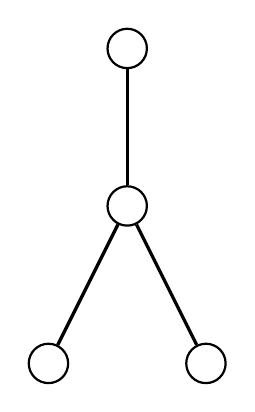
\begin{tikzpicture}[
		every edge/.style = {draw=black,very thick},
 		vrtx/.style args = {#1/#2}{% 
      	circle, draw, thick, fill=white,
      	minimum size=5mm}
                    ]
		\node(A) [vrtx=left/1] at (0, 5) {};
		\node(B) [vrtx=left/2] at (0, 3) {};
		\node(C) [vrtx=left/4] at (1, 1) {};
		\node(D) [vrtx=left/3] at (-1,1) {};

		\path   (A) edge (B)
  	 	     	(B) edge (C)        
   			    (B) edge (D);
	\end{tikzpicture}
	\captionsetup{belowskip=0pt}
    \caption*{\scriptsize Grafo original} 
    &
	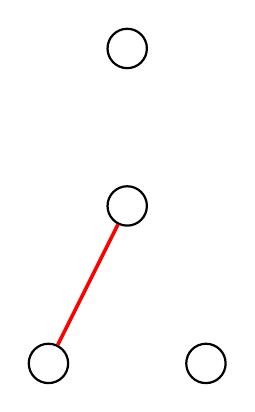
\begin{tikzpicture}[
		every edge/.style = {draw=black,very thick},
 		vrtx/.style args = {#1/#2}{% 
   	    circle, draw, thick, fill=white,
    	minimum size=5mm}
                    ]
		\node(A) [vrtx=left/1] at (0, 5) {};
		\node(B) [vrtx=left/2] at (0, 3) {};
		\node(C) [vrtx=left/4] at (1, 1) {};
		\node(D) [vrtx=left/3] at (-1,1) {};

		\path   (B) edge [color=red, line width=1.3pt] (D);
	\end{tikzpicture}
	\captionsetup{justification=centering}
	\captionsetup{belowskip=0pt}
    \caption*{\scriptsize Maximal pero no máximo}  
    &   
	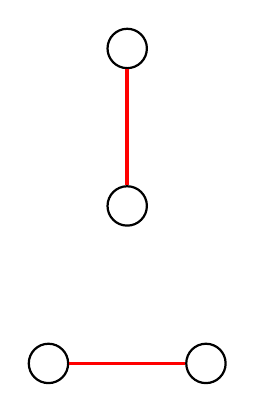
\begin{tikzpicture}[
		every edge/.style = {draw=black,very thick},
 		vrtx/.style args = {#1/#2}{%
   	    circle, draw, thick, fill=white,
      	minimum size=5mm}
                    ]
		\node(A) [vrtx=left/1] at (0, 5) {};
		\node(B) [vrtx=left/2] at (0, 3) {};
		\node(C) [vrtx=left/4] at (1, 1) {};
		\node(D) [vrtx=left/3] at (-1,1) {};

		\path   (A) edge [color=red, line width=1.3pt] (B)
        		(C) edge [color=red, line width=1.3pt] (D);
	\end{tikzpicture}
	\captionsetup{belowskip=0pt}
	\caption*{\scriptsize Apareamiento máximo}  
	\end{tabularx}
\end{figure}

\noindent El ejemplo anterior demuestra como el algoritmo podría o no encontrar el apareamiento máximo de aristas dependiendo de cual arista escoge por iteración. Este algoritmo tiene una complejidad de $O(n^2)$ ya que necesita recorrer los conjuntos disjuntos de vértices determinando si estos están marcados como visitados o no, mas el ciclo externo.

\subsection{Algoritmo Hopcroft–Karp}
Este algoritmo utiliza \textit{búsqueda por profundidad} para construir un grafo de niveles de manera alterna (se va construyendo el grafo visitando nodos de ambos subconjuntos) a partir de los vértices que no están conectados por una arista y hasta encontrar vértices ``libres". Este grafo luego se recorre con \textit{búsqueda a profundidad} a partir de los vértices que no están conectados por una arista con el fin de obtener un camino de aumentación (caminos mas cortos en el conjunto de vértices disjuntos).

\begin{center}
	\begin{algorithmic}[1]
		\STATE $M\gets \emptyset$
		\REPEAT
			\STATE $P\gets \{p_1, p_2, ..., p_k\}$
			\STATE $M\gets M \ominus \{p_1 \cup p_2 \cup ... \cup p_k\}$
		\UNTIL {$P \geq 0$}
	\RETURN $M$
	\end{algorithmic}
\end{center}

\noindent La siguiente es una version mas descriptiva del algoritmo:

\begin{center}
	\begin{algorithmic}[1]
		\STATE $M\gets \emptyset$
		\REPEAT
			\STATE \textit{búsqueda por anchura(B.F.S) para construir el grafo de niveles alternos con raíces en los vértices no apareados del conjunto V}
			\STATE \textit{Aumentar M con el conjunto maximal de caminos mas cortos obtenido al aplicar búsqueda por profundidad(D.F.S) en el grafo de niveles}
		\UNTIL {\textit{hasta que no haya mas caminos de aumentacion}}
		\RETURN $M$
	\end{algorithmic}
\end{center}

\section{Aplicaciones} \noindent
\textbf{Red de flujos(Flow network)}. Una red de flujo es un grafo dirigido donde cada arista tiene capacidad y flujo. Se usan para modelar problemas que involucran el transporte de artículos usando una red de rutas con capacidades limitadas.\\\\
\textbf{Modelado de enlaces químicos}. Mediante grafos o árboles donde los vértices representan átomos y las aristas la existencia de enlaces químicos.\\\\
\textbf{Redes neuronales artificiales}. Son modelos computacionales inspirados en el cerebro humano. Se componen de una gran cantidad de nodos conectados, cada uno de los cuales realiza una operación matemática simple. La salida de cada nodo está determinada por esta operación, así como por un conjunto de parámetros que son específicos de ese nodo. Al conectar estos nodos juntos y establecer cuidadosamente sus parámetros, se pueden aprender y calcular funciones muy complejas.

\section{Caso -- Hopcroft-Karp} \noindent
El algoritmo de Hopcroft-Karp para grafos bipartitos, utiliza \textit{búsqueda por profundidad} para construir un grafo de niveles de manera alterna (se va construyendo el grafo visitando nodos de ambos subconjuntos) a partir de los vértices que no están conectados por una arista y hasta encontrar vértices ``libres". Este grafo luego se recorre con \textit{búsqueda a profundidad} a partir de los vértices que no están conectados por una arista.

\subsection{Inicialización}
Se define e inicializan los conjuntos $M$ que almacenara las aristas que forman parte del \textit{apareamiento máximo} y $F$ que almacenara a los vértices del conjunto $W$ y que servirá para llevar control de los nodos que se visitan en ese conjunto.
\begin{center}
$M=\emptyset$; $F=\emptyset$;
\end{center}

\subsection{Primera iteración} \noindent

\begin{figure}[htb]
    \centering
    \begin{minipage}{.45\linewidth}
        \begin{subfigure}[t]{.9\linewidth}
            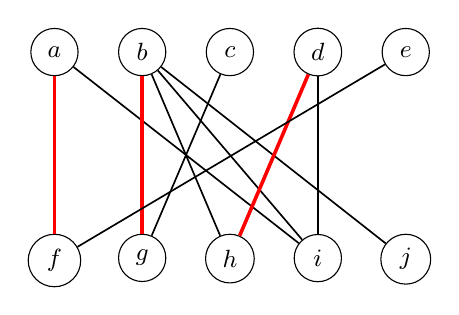
\begin{tikzpicture}[semithick]
    \tikzstyle{every state}=[
        draw = black,
        thin,
        minimum size = 6mm
    ]
    \begin{scope}[node distance=2cm and .5cm, every node/.style=state]
      \node (a) {\small $a$};
      \node (b) [right=of a] {\small $b$};
      \node (c) [right=of b] {\small $c$};
      \node (d) [right=of c] {\small $d$};
      \node (e) [right=of d] {\small $e$};
      \node (f) [below=of a] {\small $f$};
      \node (g) [below=of b] {\small $g$};
      \node (h) [below=of c] {\small $h$};
      \node (i) [below=of d] {\small $i$};
      \node (j) [below=of e] {\small $j$};
    \end{scope}
    \path[-] (a) edge [color=red, line width=1.3pt] (f)
    		 (a) edge (i)
             (b) edge [color=red, line width=1.3pt] (g)
             (b) edge (h)
             (b) edge (i)
             (b) edge (j)
             (c) edge (g)
             (d) edge [color=red, line width=1.3pt] (h)
             (e) edge (f)
             (d) edge (i);
\end{tikzpicture}
            \caption{Detail van een route}
            \label{fig:weather_filter1}
        \end{subfigure} \\\\
        \begin{subfigure}[b]{.9\linewidth}
            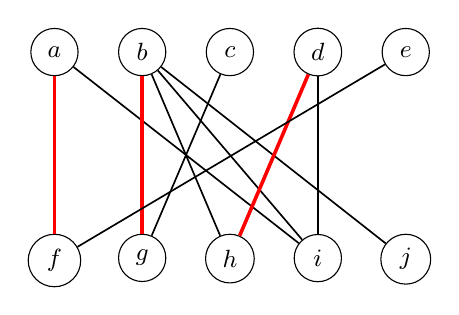
\begin{tikzpicture}[semithick]
    \tikzstyle{every state}=[
        draw = black,
        thin,
        minimum size = 6mm
    ]
    \begin{scope}[node distance=2cm and .5cm, every node/.style=state]
      \node (a) {\small $a$};
      \node (b) [right=of a] {\small $b$};
      \node (c) [right=of b] {\small $c$};
      \node (d) [right=of c] {\small $d$};
      \node (e) [right=of d] {\small $e$};
      \node (f) [below=of a] {\small $f$};
      \node (g) [below=of b] {\small $g$};
      \node (h) [below=of c] {\small $h$};
      \node (i) [below=of d] {\small $i$};
      \node (j) [below=of e] {\small $j$};
    \end{scope}
    \path[-] (a) edge [color=red, line width=1.3pt] (f)
    		 (a) edge (i)
             (b) edge [color=red, line width=1.3pt] (g)
             (b) edge (h)
             (b) edge (i)
             (b) edge (j)
             (c) edge (g)
             (d) edge [color=red, line width=1.3pt] (h)
             (e) edge (f)
             (d) edge (i);
\end{tikzpicture}
            \caption{Detail van een route}
            \label{fig:weather_filter2}
        \end{subfigure} 
    \end{minipage}
\qquad
    \begin{minipage}{.45\linewidth}
            \begin{subfigure}[t]{.9\linewidth}
                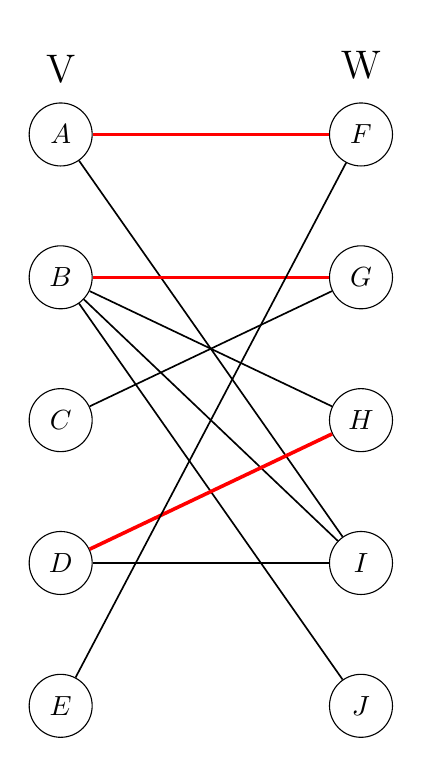
\begin{tikzpicture}[semithick]
    \tikzstyle{every state}=[
        draw = black,
        thin,
        minimum size = 8mm
    ]
    \begin{scope}[node distance=1cm and 3cm, every node/.style=state]
      \node (a) [label=above:\Large V] {$A$};
      \node (b) [below=of a] {$B$};
      \node (c) [below=of b] {$C$};
      \node (d) [below=of c] {$D$};
      \node (e) [below=of d] {$E$};
      
      \node (f) [right=of a, label=above:\Large W] {$F$};
      \node (g) [right=of b] {$G$};
      \node (h) [right=of c] {$H$};
      \node (i) [right=of d] {$I$};
      \node (j) [right=of e] {$J$};
    \end{scope}
    \path[-] (a) edge [color=red, line width=1.3pt] (f)
    		 (a) edge (i)
             (b) edge [color=red, line width=1.3pt] (g)
             (b) edge (h)
             (b) edge (i)
             (b) edge (j)
             (c) edge (g)
             (d) edge [color=red, line width=1.3pt] (h)
             (e) edge (f)
             (d) edge (i);
\end{tikzpicture}
                \caption{Weergave gezochte routes}
                \label{fig:weather_activity}
            \end{subfigure}
        \end{minipage}
    \caption{Many figures}
\end{figure}



\newpage
\nocite{*}
\bibliographystyle{ieeetr}
\bibliography{bibliography/ref}
\end{document}
